\chapter{Fo\-bwa Language}
\section{Pronunciation of Fobwa Names}
The chart that follows is of course the Pa\-co\-itz phonology. There are other phonologies such as the Joshua phonology which is much more likely to be what the actual language sounded like. There are guides and such to the Fobwa language (the good ones use the Joshua phonology) but all that suffices for this book is a pronunciation guide (if the reader cared any more about the language, they wouldn't be reading this edition).\\
\begin{tabular}
{| l  l |}
\hline
a & \underline{u}p \\
aa & f\underline{a}ther \\
i & \underline{i}n \\
ii & f\underline{ee} \\
u & b\underline{oo} \\
e & m\underline{e}t \\
ee & m\underline{ay} \\
o & n\underline{o} \\
\hline
\end{tabular}
\begin{tabular}
{| l   l |}
\hline
w & \underline{w}ait \\
m & \underline{m}other \\
n & \underline{n}ot \\
ng & si\underline{ng} \\
p & \underline{p}ay \\
t & \underline{t}ea \\
k & \underline{c}art \\
f & \underline{f}ish \\
sh & \underline{sh}oe \\
h & \underline{h}ow \\
b & \underline{b}oat \\
d & \underline{d}og \\
g & \underline{g}o \\
v & li\underline{v}e \\
z & \underline{z}oo \\
j & sei\underline{z}ure \\
\hline
\end{tabular}
\section{Properties of Fobwa}
\label{rotshift}
Alongside \emph{The Fall of King Mwe\-fu} original text, Pa\-co\-itz found some poems which scholars have attributed to Twi\-zwa. And in these poems, everything that the poet says has a most peculiar property: when the page on which Twi\-zwa's words are written is rotated 90 degrees, a second message can then be read. Not only a second though, but on subsequent rotations, a third and a fourth as well, and all of these Twi\-zwa had carefully crafted to have the meanings line up with what he wanted to say, to not be the same thing, but to be something different that expands upon the meaning of it. They call this ``rotational shift poetry.'' This is similar to ambigrams where a word becomes a different word when read in the mirror or flipped upside down, but on a scale of paragraphs instead of just individual words. To write in Fo\-bwa in such a way is a feat in itself, for even just one rotation, but to be able to do it for all four rotations and through speech alone (as Mwe\-fu implies in the original that Twi\-zwa does) takes unimaginable skill. Through speech, one needs to know where the line endings are in order to visualize what the block of text will look like, that way they know what it becomes when rotated; listening to something and being able to hear all the meanings is hard, but saying it so that all the rotations are what you want them to be is even harder. When listening, the line endings will usually be where the sentence ends most commonly are. This poetry is a very very beautiful thing, but as usual Pa\-co\-itz explains none of this and Pa\-co\-itz doesn't even make Twi\-zwa speak in verse or say things in any way that would make it obvious. Twi\-zwa's lack of poeticness in this version likely stems from Pa\-co\-itz's inability to write (poetry or otherwise).

\clearpage
\section{Basic Lexicon}
The chart above is a grossly over-simplified lexicon of the language. Each word or morpheme is just a consonant followed by a vowel. They combine to create complicated meanings based off of the basic ones.

\begin{figure}
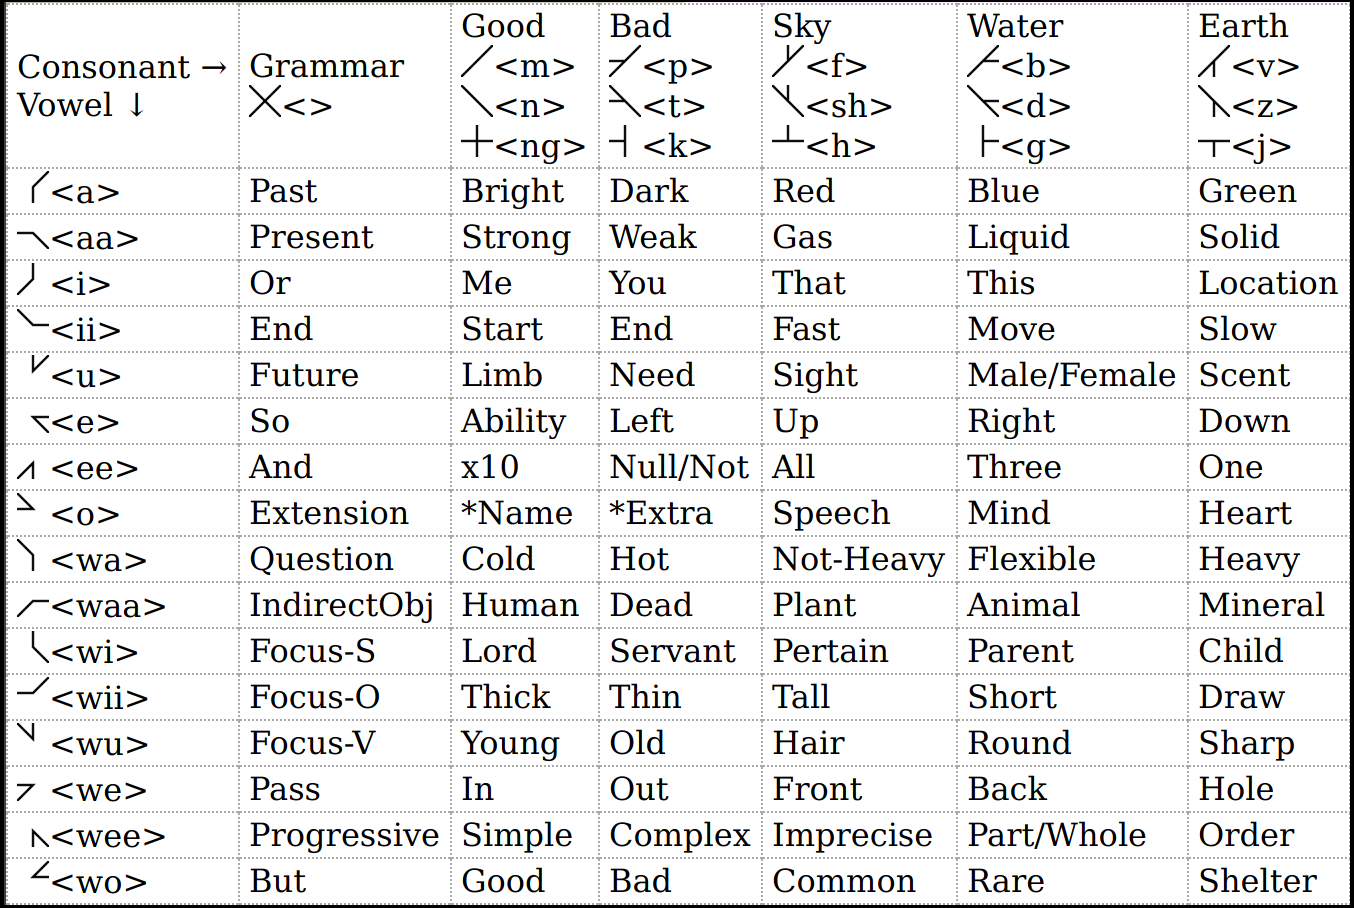
\includegraphics[width=4.0in]{language.png}
\end{figure}
\clearpage

\chapter{Origin of Fobwa Manuscripts}
In 1896, Pa\-co\-itz' worked in a restaurant located in South Dakota. But he tired of cooking and quit his job to take a vacation. (This is what Pa\-co\-itz claims, but I think it more likely that he was fired.) After a week, he found a cave in South Dakota wherein he discovered some Fobwa writing on the cave wall. Exploring further, he found some clay jars which had some poems and some historical documents as well as the original text to \emph{the Fall of King Mwe\-fu} in them. And after working on it for a couple years he had deciphered the language.

Many found it odd that Pa\-co\-itz had discovered a language that no linguist had ever seen before and that he was able to translate it without any formal training. Now, some people have theorized that Fobwa's emergence as a language, and the fact that only Pa\-co\-itz has found any major texts in that language, proves that he fabricated the language, the narratives and other documents. I shouldn't need to tell you how ridiculous this is, but since you're reading this edition instead of another, perhaps you might need me to explain. Pa\-co\-itz is constantly mistranslating phrases from the original text as well as changing various aspects about the story; if he really had written both, then he would know how to read it and would not cut out important sections from it. If Pa\-co\-itz had written the original text, then one would expect the original to be shorter both because it's a lot more work to write in Fobwa and because Pa\-co\-itz only seem to care about his English translation.

Pa\-co\-itz is just not creative enough to come up with anything original, let alone create an elaborate well-thought-out hoax to purport a translation of what would be fake documents written in a fake language.

Not a single scholar of any standing finds any of \emph{the Elevated Pa\-co\-itz Doctrine} (As some call it) to have even an inkling of credibility. The texts have all the evidence of older productions; Joshua Greenberg confirmed the works (via carbon dating some excess paper) to be at least 1,300 years old. So it is highly probable that Fobwa, and \emph{The Fall of King Mwe\-fu} are historical works and not apocryphal.


